\section{Background}

\subsection{Pig-Latin Compilation}
\begin{frame}{Pig Latin Compilation}
\begin{enumerate}
	\item Pig program verification, type checking, schema inference.
	\item Pig program to logical plan (1-1 mapping).
	\item Logical plan to physical plan (map to physical operators).
	\item Physical plan to MapReduce (try to minimize stages).
\end{enumerate}
\end{frame}

%\subsection{MapReduce Execution Model}
%\begin{frame}{MapReduce Execution Model}
%\begin{itemize}
%	\item Map: Produces a stream of data items annotated with keys.
%	\item Local Sort: Orders the data at each machine by key.
%	\item Combiner: Performs partial aggregation on the locally ordered data.
%	\item Shuffle: Redistributes the data to achieve global ordering.
%	\item Merge/Combine: All data received at a particular machine is combined
%          into a single stream in merge stage.
%	\item Reduce: Finally the reduce stage processes the data associated with
%          each key and performs aggregation of the output results.
%\end{itemize}
%\end{frame}
%
%\begin{frame}{MapReduce Execution Model}
%\centerline{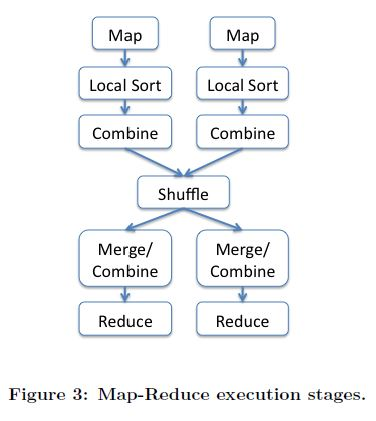
\includegraphics[scale=0.5]{Images/MapReduce_Execution.JPG}}
%\let\thefootnote\relax\footnotetext{\tiny\citet[VLDB][]{gates2009building}}
%\end{frame}

%\subsection{Pig Latin's Logical Plan}
%\begin{frame}{Logical Plan Structure}
%\begin{itemize}
%	\item A Pig Latin program is a sequence of steps, each of which carries out
%          a single transformation.
%	\item Each Pig Latin program is translated to a logical plan
%	\item Pig then translates the logical plan to a physical plan and embeds
%          each physical operator inside a MapReduce stage to arrive at the
%          MapReduce plan.
%\end{itemize}
%\end{frame}

\subsection{PigLatin - Logical Plan}
\begin{frame}{Logical Plan}
\centerline{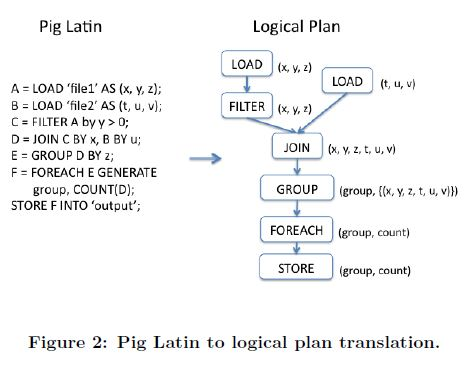
\includegraphics[scale=0.55]{Images/PigLatin.JPG}}
\let\thefootnote\relax\footnotetext{\tiny \citet[VLDB][]{gates2009building}}
\end{frame}

%\subsection{Generating MapReduce Jobs}
%\begin{frame}{Logical-MapReduce}
%\begin{itemize}
%	\item Pig translates the logical plan to a physical plan
%	\item Logical (CO)GROUP operator translates to - local rearrange, global
%          rearrange and package.
%	\item The JOIN is handled either with a COGROUP followed by a FOREACH or
%          fragment replicate join.
%	\item After the physical plan is generated Pig assigns physical operators to
%          Hadoop Stages
%\end{itemize}
%\end{frame}

\subsection{Logical Plan - Physical Plan}
\begin{frame}
\centerline{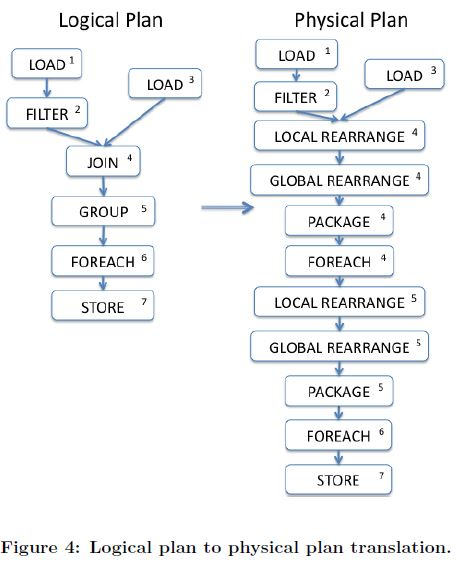
\includegraphics[scale=0.40]{Images/Logical_Physical.JPG} }
\let\thefootnote\relax\footnotetext{\tiny \citet[VLDB][]{gates2009building}}
\end{frame}

\subsection{Physical Plan - Map Reduce}
\begin{frame}
\centerline{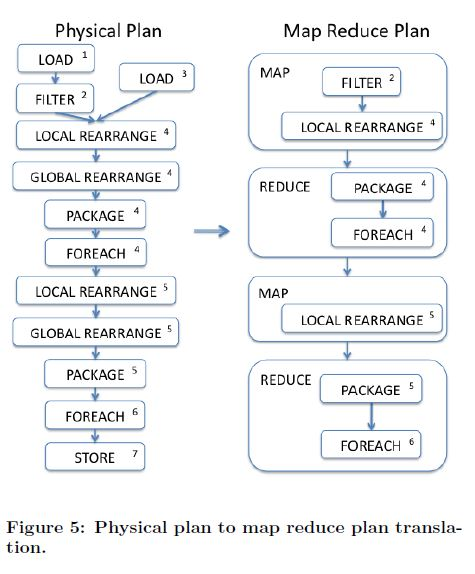
\includegraphics[scale=0.40]{Images/Physical_MapReduce.JPG}}
\let\thefootnote\relax\footnotetext{\tiny \citet[VLDB][]{gates2009building}}
\end{frame}

%\begin{frame}{Pig to MapReduce}
%\begin{itemize}
%	\item Pig compiles programs written in Pig Latin
%	\item Ultimately translates to Map-Reduce tasks
%	\item Pig also operates on local mode running on a single machine without
%          map-reduce
%	\item There lies an equivalence between PigLatin and MapReduce operational
%          semantics
%	\item The equivalence needs to be formalized and correctness needs to be
%          proved
%\end{itemize}
%\end{frame}


%\subsection{Three Main Papers}
%
%\begin{frame}{\citet[VLDB][]{gates2009building}}
%\emph{Building a HighLevel Dataflow System on top of MapReduce: The Pig
%Experience}:
%\begin{itemize}
%	\item This paper outlines the compilation phase of PigLatin programs and how
%          the logical plan of PigLatin is translated to actual Hadoop map-reduce
%          tasks.
%	\item But neither the semantics nor the compilation to map-reduce framework
%          have been formalized with proof of correctness.
%\end{itemize}
%\end{frame}
%
%\begin{frame}{\citet[SEFM]{ono2011using}}
%\emph{Using Coq in Specification and Program Extraction of Hadoop MapReduce
%Applications}
%\begin{itemize}
%    \item Constructed formal model of MapReduce computation in Coq where:
%    \begin{itemize}
%        \item Model user-defined map/reduce as Coq functions
%        \item Application specifications are defined as invariants
%    \end{itemize}
%	\item Constructed formal model of the (previously informally specified)
%          Hadoop libraries
%	\item Using these, they prove the correctness of some example MapReduce
%          applications.
%    \item Future Work: Investigate a more MapReduce applications
%\end{itemize}
%\end{frame}
%
%\begin{frame}{\citet[Journal of Automated Reasoning][]{leroy2009formally}}
%\emph{A formally verified compiler back-end}
%\begin{itemize}
%	\item Compcert: Formally verified compiler from Cminor to PPC assembly.
%    \item Programmed and proven sound using Coq.
%    \item Lots of background on compiler verification.
%\end{itemize}
%\end{frame}
